\documentclass[tikz]{standalone}
\usepackage{tikz}
\usetikzlibrary{calc}
\usetikzlibrary{positioning}
\usetikzlibrary{fit}
\usetikzlibrary{backgrounds}

\definecolor{lightGreen}{HTML}{d5e8d4}
\definecolor{lightYellow}{HTML}{fff2cc}
\definecolor{lightGray}{HTML}{f5f5f5}
\definecolor{lightRed}{HTML}{ff9999}
\definecolor{lightBlue}{HTML}{d5e5fc}
\definecolor{lightCyan}{HTML}{a7dfe3}
\pgfdeclarelayer{main_bg}
\pgfdeclarelayer{back_bg}
\pgfsetlayers{main_bg,back_bg,main}

\newcommand{\metarect}[7]{
    \begin{scope}
        \node (#1) [rectangle, draw, text width=\rectWidth, minimum width=\rectWidth, minimum height=\rectHeight, #7] {};
        \node (#1_upper) [rectangle, draw, fill=#6, text width=\rectWidth, minimum width=\rectWidth, minimum height=\rectHeight*0.5, below=0.0pt of #1.north, anchor=north] {#2};
        \node (#1_middle) [rectangle, draw, fill=white, font=\tiny, text width=\rectWidth, minimum width=\rectWidth, minimum height=\rectHeight*0.25, below=-\the\pgflinewidth of #1_upper] {#3};
        \node (#1_bleft) [rectangle, draw, fill=white, font=\tiny, text width=\rectWidth*0.35, minimum width=\rectWidth*0.35, minimum height=\rectHeight*0.25, below=-\the\pgflinewidth of #1_middle.south west, anchor=north west] {#4};
        \node (#1_bright) [rectangle, draw, fill=white, font=\tiny, text width=\rectWidth*0.65, minimum width=\rectWidth*0.65, minimum height=\rectHeight*0.25, right=-\the\pgflinewidth of #1_bleft] {#5};
    \end{scope}
}

\newcommand{\metarectvec}[5]{
    \begin{scope}
        \node (#1) [draw, rectangle, text width=\rectWidth, minimum width=\rectWidth, minimum height=\rectHeight*0.25, #5] {};
        \node (#1_left) [draw, rectangle, fill=#4, font=\footnotesize, text width=\rectWidth*0.4, minimum width=\rectWidth*0.4, minimum height=\rectHeight*0.25, below=0.0pt of #1.north west, anchor=north west] {#2};
        \node (#1_right) [draw, rectangle, fill=white, font=\tiny, text width=\rectWidth*0.6, minimum width=\rectWidth*0.6, minimum height=\rectHeight*0.25, right=-\the\pgflinewidth of #1_left] {#3};
    \end{scope}
}

\begin{document}
    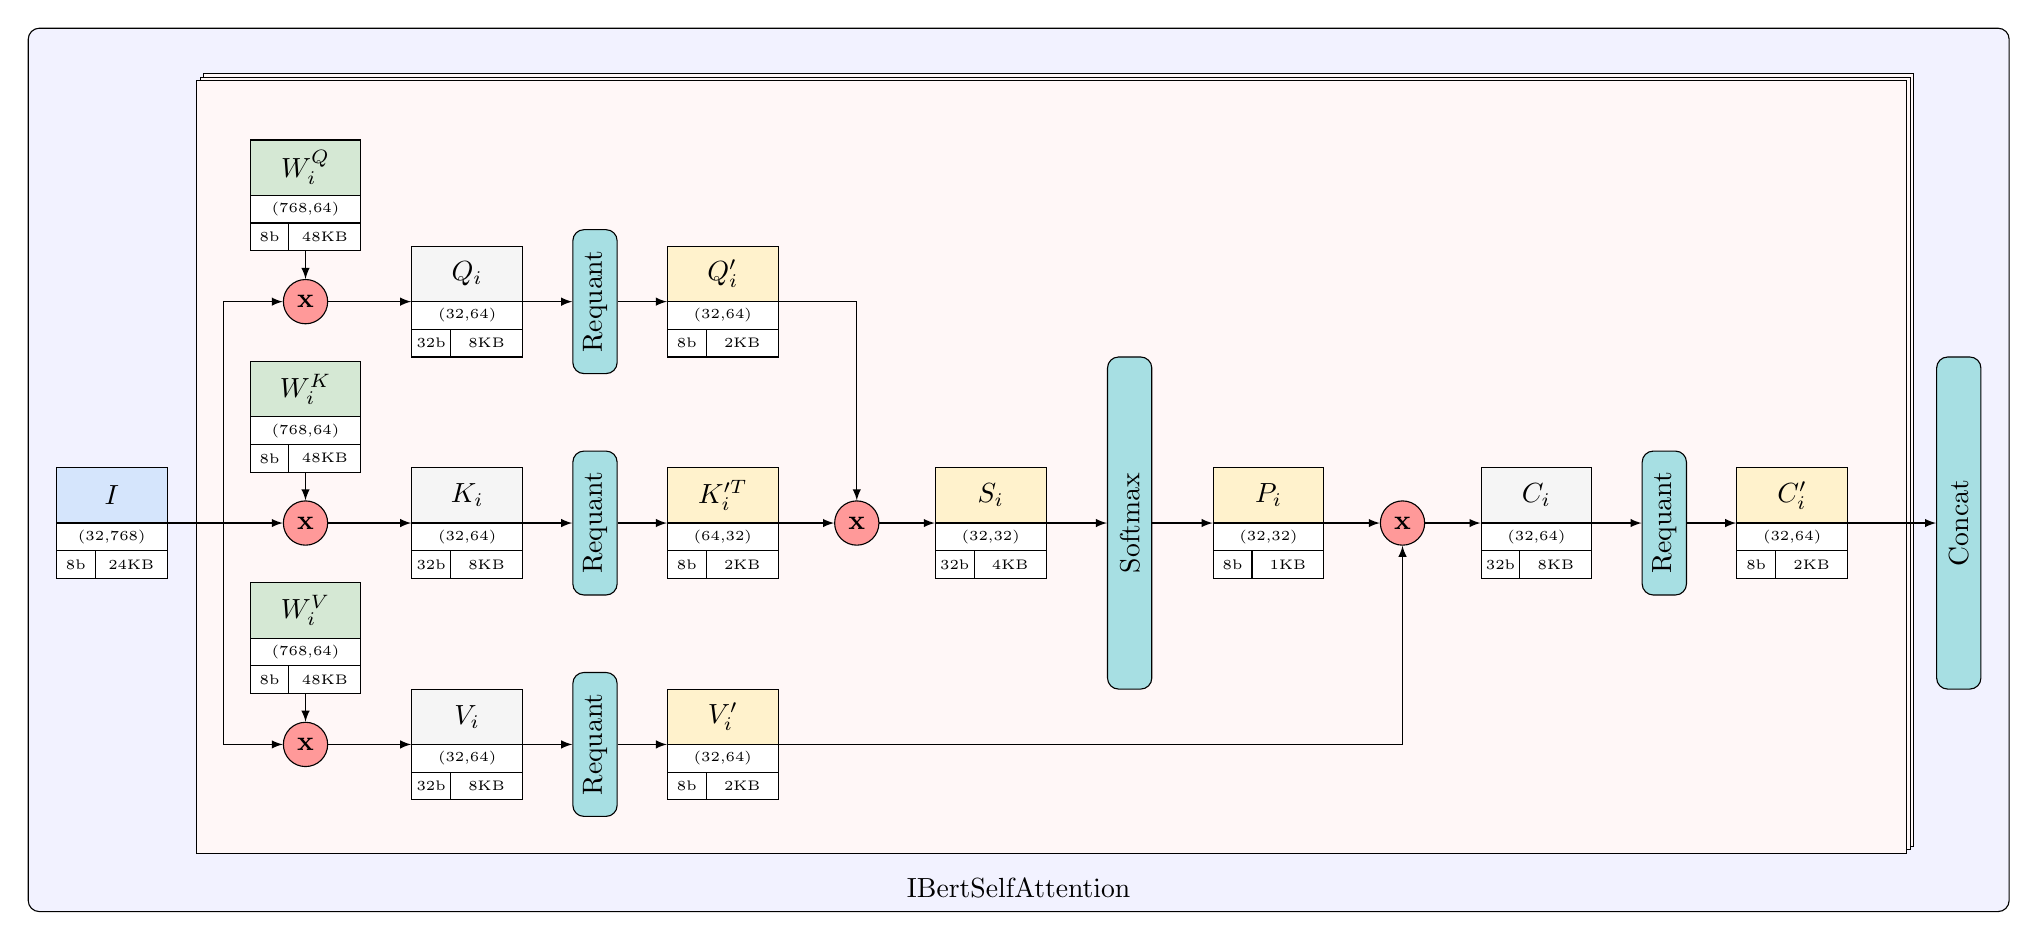
\begin{tikzpicture}[inner sep=0.0 pt, align=center]
    \pgfmathsetmacro{\rectWidth}{40}
    \pgfmathsetmacro{\rectHeight}{40}

    \metarect{layer_input}{$I$}{(32,768)}{8b}{24KB}{lightBlue}{}

    \pgfmathsetmacro{\multSize}{16 pt}
    \node [draw, circle, fill=lightRed, minimum size=\multSize, right=\rectWidth*1.75pt of layer_input.center, anchor=center] (mult1) {\textbf{x}};
    \node [draw, circle, fill=lightRed, minimum size=\multSize, above=\rectHeight*2pt of mult1.center, anchor=center] (mult2) {\textbf{x}};
    \node [draw, circle, fill=lightRed, minimum size=\multSize, below=\rectHeight*2pt of mult1.center, anchor=center] (mult3) {\textbf{x}};

    \metarect{weight_Q}{$W_i^Q$}{(768,64)}{8b}{48KB}{lightGreen}{above=\rectHeight*0.25pt of mult2}
    \metarect{weight_K}{$W_i^K$}{(768,64)}{8b}{48KB}{lightGreen}{above=\rectHeight*0.25pt of mult1}
    \metarect{weight_V}{$W_i^V$}{(768,64)}{8b}{48KB}{lightGreen}{above=\rectHeight*0.25pt of mult3}

    \draw [-latex] (weight_Q.south) -- (mult2.north);
    \draw [-latex] (weight_K.south) -- (mult1.north);
    \draw [-latex] (weight_V.south) -- (mult3.north);

    \draw [-latex] (layer_input.east) -| ([xshift=\rectWidth*0.5 pt]layer_input.east) |- (mult2.west);
    \draw [-latex] (layer_input.east) -| ([xshift=\rectWidth*0.5 pt]layer_input.east) |- (mult1.west);
    \draw [-latex] (layer_input.east) -| ([xshift=\rectWidth*0.5 pt]layer_input.east) |- (mult3.west);

    \metarect{mixQ32b}{$Q_i$}{(32,64)}{32b}{8KB}{lightGray}{right=\rectWidth*0.75pt of mult2}
    \metarect{mixK32b}{$K_i$}{(32,64)}{32b}{8KB}{lightGray}{right=\rectWidth*0.75pt of mult1}
    \metarect{mixV32b}{$V_i$}{(32,64)}{32b}{8KB}{lightGray}{right=\rectWidth*0.75pt of mult3}

    \draw [-latex] (mult2.east) -- (mixQ32b.west);
    \draw [-latex] (mult1.east) -- (mixK32b.west);
    \draw [-latex] (mult3.east) -- (mixV32b.west);

    \node [draw, fill=lightCyan, rounded corners, minimum width=\rectHeight*1.3, minimum height=\rectWidth*0.4, rotate=90, right=\rectWidth*0.65pt of mixQ32b, anchor=center] (reqQ) {Requant};
    \node [draw, fill=lightCyan, rounded corners, minimum width=\rectHeight*1.3, minimum height=\rectWidth*0.4, rotate=90, right=\rectWidth*0.65pt of mixK32b, anchor=center] (reqK) {Requant};
    \node [draw, fill=lightCyan, rounded corners, minimum width=\rectHeight*1.3, minimum height=\rectWidth*0.4, rotate=90, right=\rectWidth*0.65pt of mixV32b, anchor=center] (reqV) {Requant};

    \draw [-latex] (mixQ32b.east) -- (reqQ.north);
    \draw [-latex] (mixK32b.east) -- (reqK.north);
    \draw [-latex] (mixV32b.east) -- (reqV.north);

    \metarect{mixQ8b}{$Q_i'$}{(32,64)}{8b}{2KB}{lightYellow}{right=\rectWidth*0.65pt of reqQ.center}
    \metarect{mixK8b}{$K_i'^T$}{(64,32)}{8b}{2KB}{lightYellow}{right=\rectWidth*0.65pt of reqK.center}
    \metarect{mixV8b}{$V_i'$}{(32,64)}{8b}{2KB}{lightYellow}{right=\rectWidth*0.65pt of reqV.center}

    \draw [-latex] (reqQ.south) -- (mixQ8b.west);
    \draw [-latex] (reqK.south) -- (mixK8b.west);
    \draw [-latex] (reqV.south) -- (mixV8b.west);

    \node [draw, circle, fill=lightRed, minimum size=\multSize, right=\rectWidth*0.5pt of mixK8b] (multSelf1) {\textbf{x}};
    \metarect{Si}{$S_i$}{(32,32)}{32b}{4KB}{lightYellow}{right=\rectWidth*0.5pt of multSelf1}

    \draw [-latex] (mixQ8b.east) -| (multSelf1.north);
    \draw [-latex] (mixK8b.east) -- (multSelf1.west);
    \draw [-latex] (multSelf1.east) -- (Si.west);

    \node [draw, fill=lightCyan, rounded corners, minimum width=\rectHeight*3, minimum height=\rectWidth*0.4, rotate=90, right=\rectWidth*0.75pt of Si, anchor=center] (softmax) {Softmax};

    \metarect{Pi}{$P_i$}{(32,32)}{8b}{1KB}{lightYellow}{right=\rectWidth*0.75pt of softmax.center}
    \node [draw, circle, fill=lightRed, minimum size=\multSize, right=\rectWidth*0.5pt of Pi] (multSelf2) {\textbf{x}};
    \metarect{Ci}{$C_i$}{(32,64)}{32b}{8KB}{lightGray}{right=\rectWidth*0.5pt of multSelf2}
    \node [draw, fill=lightCyan, rounded corners, minimum width=\rectHeight*1.3, minimum height=\rectWidth*0.4, rotate=90, right=\rectWidth*0.65pt of Ci, anchor=center] (reqC) {Requant};
    \metarect{Ci8b}{$C_i'$}{(32,64)}{8b}{2KB}{lightYellow}{right=\rectWidth*0.65pt of reqC.center}

    \draw [-latex] (Si.east) -- (softmax.north);
    \draw [-latex] (softmax.south) -- (Pi.west);
    \draw [-latex] (Pi.east) -- (multSelf2.west);
    
    \draw [-latex] (mixV8b.east) -| (multSelf2.south);
    \draw [-latex] (multSelf2.east) -- (Ci.west);
    \draw [-latex] (Ci.east) -- (reqC.north);
    \draw [-latex] (reqC.south) -- (Ci8b.west);

    \begin{pgfonlayer}{main_bg}
        \node (self_rect) [draw, rectangle, fill=black!3, inner sep=20pt, fit=(weight_Q)(weight_K)(weight_V)(mixQ32b)(mixV32b)(Ci8b)] {};
        \begin{pgfonlayer}{back_bg}
            \foreach \x in {3,...,1} {
                \node [draw, rectangle, fill=red!3, fit=(self_rect), above right=\x*1.25pt-\the\pgflinewidth and \x*1.25pt-\the\pgflinewidth of self_rect.south west] {};
            }
        \end{pgfonlayer}
    \end{pgfonlayer}

    \node [draw, fill=lightCyan, rounded corners, minimum width=\rectHeight*3, minimum height=\rectWidth*0.4, rotate=90, right=\rectWidth*1pt of Ci8b, anchor=center] (concat) {Concat};
    \draw [-latex] (Ci8b.east) -- (concat.north);

    \begin{pgfonlayer}{main_bg}
        % fill=red!3
        \node (SelfAtt) [draw, rectangle, fill=blue!5, rounded corners, inner xsep=10pt, inner ysep=20pt, fit=(layer_input)(self_rect)(concat)] {};
        \node (SelfAttText) [above=5.0pt of SelfAtt.south] {IBertSelfAttention};

        % \node (all) [draw, rectangle, inner xsep=20pt, inner ysep=40pt, fit=(layer_input)(weight_Q)(weight_K)(weight_V)(mixQ32b)(mixV32b)(Ci8b)(concat)] {};
    \end{pgfonlayer}


    \end{tikzpicture}

\end{document}
